\documentclass[12pt]{article}
\usepackage{amsmath} % AMS Math Package
\usepackage{bm}
\usepackage{amsthm} % Theorem Formatting
\usepackage{amssymb}    % Math symbols such as \mathbb
\usepackage{graphicx} % Allows for eps images
\usepackage[dvips,letterpaper,margin=1in,bottom=0.7in]{geometry}
\usepackage{tensor}
\usepackage{amsmath}
\usepackage{siunitx}
\usepackage{physics}
\usepackage{amsmath, amssymb, graphics, setspace}
\usepackage{listings}
\usepackage{color}

\definecolor{dkgreen}{rgb}{0,0.6,0}
\definecolor{gray}{rgb}{0.5,0.5,0.5}
\definecolor{mauve}{rgb}{0.58,0,0.82}

\lstset{frame=tb,
  language=Java,
  aboveskip=3mm,
  belowskip=3mm,
  showstringspaces=false,
  columns=flexible,
  basicstyle={\small\ttfamily},
  numbers=none,
  numberstyle=\tiny\color{gray},
  keywordstyle=\color{blue},
  commentstyle=\color{dkgreen},
  stringstyle=\color{mauve},
  breaklines=true,
  breakatwhitespace=true,
  tabsize=3
}

\newcommand{\mathsym}[1]{{}}
\newcommand{\unicode}[1]{{}}

\newcounter{mathematicapage}

\newtheorem{p}{Problem}
\usepackage{cancel}
\newtheorem*{lem}{Lemma}
\theoremstyle{definition}
\newtheorem*{dfn}{Definition}
 \newenvironment{s}{%\small%
        \begin{trivlist} \item \textbf{Solution}. }{%
            \hspace*{\fill} $\blacksquare$\end{trivlist}}%

\makeatletter
% we use \prefix@<level> only if it is defined
\renewcommand{\@seccntformat}[1]{%
  \ifcsname prefix@#1\endcsname
    \csname prefix@#1\endcsname
  \else
    \csname the#1\endcsname\quad
  \fi}
% define \prefix@section
\newcommand\prefix@section{}
\newcommand{\prefix@subsection}{}
\newcommand{\prefix@subsubsection}{\thesubsubsection\ - }
\renewcommand{\thesubsection}{\arabic{subsection}}
\makeatother

\begin{document}

 {\noindent\Huge\bf  \\[0.5\baselineskip] {\fontfamily{cmr}\selectfont  Project 2}         }\\[2\baselineskip] % Title
{ {\bf \fontfamily{cmr}\selectfont Quantum Mechanics}\\ {\textit{\fontfamily{cmr}\selectfont     \today}}}~~~~~~~~~~~~~~~~~~~~~~~~~~~~~~~~~~~~~~~~~~~~~~~~~~~~~~~~~~~~~~~~~~~~~~~~~~~~~    
{\large \textsc{C Seitz}
\\[1.4\baselineskip] 

\section{Finite Differences Method}

For all time-dependent problems e.g., superposition states or time-dependent potentials, I use the finite difference in the time domain (FDTD) method to solve Schrodinger's equation. The algorithm is well-known, so I will just sketch the major result I use here. The idea is the break up the time-dependent Schrodinger equation into coupled differential equations for the real and imaginary parts of the wavefunction. 

Let $\ell$ be a discrete spatial coordinate and $m,n$ index time for the real $\psi_{R}(\ell)$ and imaginary $\psi_{I}(\ell)$ parts of the wavefunction, respectively. The update equations are

\begin{align*}
\frac{1}{\Delta \tau}\left(\psi_{I}^{n+1}(\ell)-\psi_{I}^{n}(\ell)\right) &= \eta\left(\psi_{R}^{m}(\ell + 1) - 2\psi_{R}^{m}(\ell)+ \psi_{R}^{m}(\ell -1 )\right) - V(\ell)\psi_{R}^{m}(\ell)
\end{align*}

\begin{align*}
\frac{1}{\Delta \tau}\left(\psi_{R}^{m+1}(\ell)-\psi_{R}^{m}(\ell)\right) &= -\eta\left(\psi_{I}^{n}(\ell + 1) - 2\psi_{I}^{n}(\ell)+ \psi_{I}^{n}(\ell -1 )\right) - V(\ell)\psi_{I}^{n}(\ell)\\
\end{align*}

where $\tau = t/\hbar$ and $\eta = \frac{\hbar^{2}}{2m\Delta x^{2}}$ (and we set $\eta=1$) is the hopping parameter. You solve the system numerically by alternatively updating the real and imaginary wavefunctions in time. Suppose the initial state is $\ket{\alpha} = \frac{1}{\sqrt{2}}\left(\ket{0} + \ket{1}\right)$ where $\ket{0}$ and $\ket{1}$ are the ground state and first excited state for the infinite square well. Then we find the position representation $\bra{i}\ket{0}$ and $\bra{i}\ket{1}$ by solving the time-independent Schrodinger equation as in Project 1. We then can construct $\bra{i}\ket{\alpha}$, which is purely real, and assign this as the initial condition $\psi_{R}^{0}(\ell)$.

\section{Part 1}

\subsection{Answers}

\noindent \textbf{(A)} Since the wavefunction is a superposition of eigenkets, I expect the probability density to change in time, probably in an oscillatory fashion.\\
\noindent \textbf{(B)} The time scale should depend on the energies of the eigenkets of the superposition\\
\noindent \textbf{(C)} See Figure 1 for FDTD simulation of the infinite and finite square wells\\
\noindent \textbf{(D)} For any superposition state, we can write

\begin{align*}
\langle x \rangle &= \sum_{a'}\sum_{a''}c_{a'}^{*}c_{a''}\bra{a'}x\ket{a''}\exp\left(\frac{-i(E_{a''}-E_{a'})t}{\hbar}\right)
\end{align*}

which in this particular case (using $\tau = t/\hbar$) is
\begin{align*}
\langle x \rangle = \frac{1}{2}\left(\bra{0}x\ket{1}\exp\left(i\Delta E\tau\right) + \bra{1}x\ket{0}\exp\left(-i\Delta E\tau\right)\right)\\
\end{align*}


The angular frequency will be higher for the finite square well because $\Delta E = E_{1}-E_{0}$ is larger see the derivative of the eigenvalue spectrum in Figure 1).


\noindent \textbf{(E)} See email attachments for the gif animation corresponding to the simulations in Figure 1


\begin{figure}
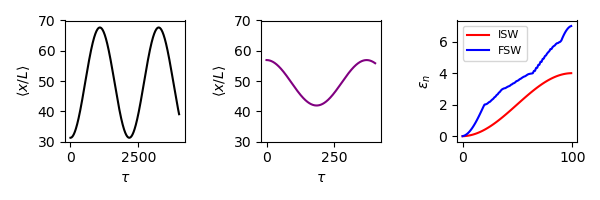
\includegraphics[scale=1]{Figure_1.png}
\centering
\caption{Expectation values of position as a function of time for the infinite (left) and finite (middle) square well, plus the eigenvalue spectrum for both (right). $d\tau = 0.01, \eta =1, N_{x}=100, N_{t} = 4\times 10^{5}$}
\end{figure}


\section{Part 2}

\begin{figure}
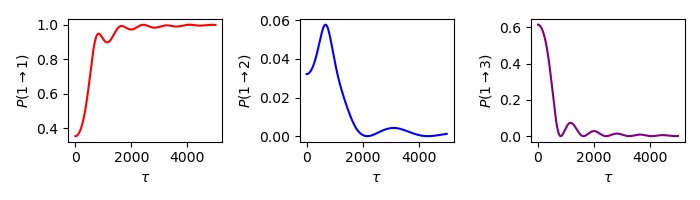
\includegraphics[scale=1]{Figure_2.png}
\centering
\caption{Transition probability $P(1\rightarrow 1) = |c_{1}(t)|^{2}$ (left) computed with Equation 2, $P(1\rightarrow 2) = |c_{2}(t)|^{2}$ (middle), and $P(1\rightarrow 3) = |c_{3}(t)|^{2}$ (right), both computed with Equation 1. Expansion coefficients were renormalized at each time step. $d\tau = 0.1, N_{t} = 5\times 10^{4}$}
\end{figure}


\subsection{Time-dependent peturbation theory for a constant perturbation}


We are using the time-dependent Hamiltonian

\begin{align*}
H(x,t) = H_{0}(x) + \lambda(1-e^{-t/\tau})V(x)
\end{align*}

where $V(x)$ is the finite square well potential. We are assuming that $\tau\rightarrow\infty$ so the potentially turns on exactly at $t=0$, giving a \textbf{constant perturbation}. 

\subsection{Answers}


\noindent \textbf{(F)} If $\lambda = 0$, we do not expect $\langle x/L\rangle$ to oscillate because $H(t) = H_{0}$ and $\ket{\psi} = \ket{i}$ which is an eigenstate of $H_{0}$.\\
\noindent \textbf{(G)} If $\lambda \neq 0$, we do expect $\langle x/L\rangle$ to oscillate because turning on the potential $V(x)$ makes $\ket{\psi}$ a superposition of eigenkets of the $H(t) = H_{0} + \lambda V(x)$\\
\noindent \textbf{(H)}

\begin{figure}
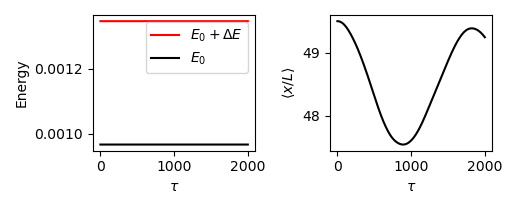
\includegraphics[scale=1]{Figure_3.png}
\centering
\caption{Analytical calculation of the expectation value of position (left) and energy (right)}
\end{figure}

Now, we are told that we start in the ground state of $H_{0}$, which is the Hamiltonian for an infinite square well, i.e. $\ket{\psi(0} = \ket{i} = \ket{1}$. recall that in time-dependent first order perturbation theory, Schrodinger's equation becomes

\begin{align*}
i\hbar\frac{d}{dt}c_{n}^{(0)}(t) &= 0\\
i\hbar\frac{d}{dt}c_{n}^{(1)}(t) &= \sum_{i}V_{ni}e^{i\omega_{ni}t}c_{i}^{(0)}(t)
\end{align*}

where $V_{ni} = \bra{n}V\ket{i}$ and $c_{n}(t)$ is the expansion coefficient for \textbf{unperturbed} energy eigenket $\ket{n}$. In general, expansion coefficients for energy eigenkets are, to first order

\begin{align*}
c_{n}(t) &\approx c_{n}^{(0)}(t) + \lambda c_{n}^{(1)}(t)\\
&= \delta_{ni} - \frac{i\lambda}{\hbar}\int_{0}^{t}V_{ni}e^{i\omega_{ni}t}dt
\end{align*}

To first order, the transition probabilities $P(i\rightarrow n) = |c_{n}^{(1)}(t)|^{2}$. From the expression above, we have

\begin{align*}
c_{n}^{(1)}(t) &= -\frac{i}{\hbar}\int_{0}^{t}V_{ni} e^{i\omega_{ni}t}dt\\
&= \frac{V_{ni}}{E_{n}-E_{i}}(1-e^{i\omega_{ni}t})
\end{align*}

Therefore,

\begin{align}
P(i\rightarrow n) &= \frac{4|V_{ni}|^{2}}{|E_{n}-E_{i}|^{2}}\sin^{2}\left(\frac{(E_{n}-E_{i})t}{2\hbar}\right)
\end{align}

Clearly the transition probability oscillates but the amplitude of this oscillation is small provided the magnitude of the transition matrix element $V_{ni}$ of the perturbation is small compared to the unperturbed energy difference between the initial and final states. However, if $E_{n} = E_{i}$, the transition probability grows quadratically in time


\begin{align}
P(i\rightarrow n) &= |V_{ni}|^{2}t^{2}
\end{align}

\noindent \textbf{(I)} To compute the wavefunction $\bra{i}\ket{\alpha(\tau)}$ we need both the magnitude and phase of the first order corrections to the expansion coefficients: 

\begin{align*}
c_{n}(t) &\approx c_{n}^{(0)}(t) + \lambda c_{n}^{(1)}(t)\\
&= \delta_{ni} + \frac{V_{ni}}{E_{n}-E_{i}}(1-e^{i\omega_{ni}t})
\end{align*}

We can ensure that $\bra{i}\ket{\alpha(\tau)}$ is normalized by dividing the coefficients by $\sum_{n}|c_{n}(\tau)|^{2}$ at each $\tau$.


\noindent \textbf{(J)} I wasn't able to get this part to work correctly with my FDTD method, so my animation is generated by computing the coefficients from part (I) directly and constructing the superposition:

\begin{align*}
\bra{i}\ket{\alpha(\tau)} = c_{1}(t)\psi_{1}(\ell) + c_{2}(t)\psi_{2}(\ell) + c_{3}(t)\psi_{3}(\ell)
\end{align*}

where $\psi_{n}(\ell)$ are orthonormal.

\noindent \textbf{(K)} As $\tau\rightarrow \infty$ we should have the wavefunction approach that of the ground state i.e, $\bra{i}\ket{\alpha(\tau)}\rightarrow \bra{i}\ket{1}$, because as you can see in Figure 2, the transition probability $P(1\rightarrow 1)$ grows quadratically in time while the other transition probabilities oscillate sinusoidally. 
\\
\noindent \textbf{(L)} The expectation value $\langle x/L\rangle$ is plotted as a function of time in Figure 3. When the potential is turned on, the particle goes from a stationary state to a superposition and then slowly back to a stationary state for the same reason as in (K).\\
\noindent \textbf{(M)}The expectation value $\langle H\rangle$ is plotted as a function of time in Figure 3.\\
\noindent \textbf{(N)} Energy does not need to be conserved by the uncertainty principle for energy and time $\Delta E\Delta t \geq \hbar/2$ which in this case is $\Delta E\Delta \tau \geq 1/2$. Since time is a parameter in nonrelativistic quantum mechanics, energy conservation can be violated over short time scales. \\
\noindent \textbf{(O)} At long times $\langle H_{0} \rangle = E_{0}$, so no energy is transferred to the system\\



\clearpage


\begin{lstlisting}
import numpy as np
import matplotlib.pyplot as plt
from numpy import linalg as LA
from plt2array import plt2array
from skimage.io import imsave

class FDTDSolver:
    def __init__(self,Nx,Nt,V,psi_r0,psi_i0,dir,plot=True,plot_iter_num=10,dt=0.1,name='sim',H=None):
        self.Nt = Nt
        self.Nx = Nx
        self.V = V
        self.psi_r0 = psi_r0
        self.psi_i0 = psi_i0
        self.psi_r = psi_r0
        self.psi_i = psi_i0
        self.psi_r = np.pad(self.psi_r, (1,1))
        self.psi_i = np.pad(self.psi_i, (1,1))
        self.prob = np.zeros((Nx,Nt))
        self.prob[:,0] = self.psi_r[1:-1]**2 + self.psi_i[1:-1]**2
        self.c1 = dt
        self.c2 = dt
        self.dir = dir
        self.plot_iter_num = plot_iter_num
        self.plot = plot
        self.name = name
        self.dt = dt
        self.H = H
        self.Etau = np.zeros((Nt,))

    def compute_energy(self,t):
        psi = self.psi_r[1:-1] + self.psi_i[1:-1]*1j
        self.Etau[t] = np.conjugate(psi) @ self.H @ psi

    def plot_init_(self):
        fig, ax = plt.subplots(figsize=(3,1))
        ax.plot(self.psi_r0,color='red')
        ax.plot(self.psi_i0,color='blue')
        plt.tight_layout()
        plt.show()

    def plot_iter(self,t):
        fig, ax = plt.subplots()
        ax1 = ax.twinx()
        ax.set_ylim([-0.1,0.1])
        ax1.set_ylim([-2*self.V.max(),2*self.V.max()])
        ax.plot(self.psi_r,color='red',label=r'$\psi_{R}$')
        ax.plot(self.psi_i,color='blue',label=r'$\psi_{I}$')
        ax.plot(self.psi_i**2 + self.psi_r**2,color='purple',label=r'$|\psi|^{2}$')
        ax1.plot(self.V[:,t],color='black',label=r'$V(x)$')
        ax1.set_ylabel('V(x)')
        ax.text(0.05, 0.95, r'$\tau$' + f'={self.dt*t}', transform=ax.transAxes, fontsize=14,
        verticalalignment='top')
        ax.legend()
        plt.tight_layout()
        rgb_array = plt2array(fig)
        imsave(self.dir+f'{t}_{self.name}.tif',rgb_array)
        plt.close()

    def update_r(self,t):
        for n in range(1,self.Nx+1):
            self.psi_r[n] = self.psi_r[n]-\
            self.c1*(self.psi_i[n+1] - 2*self.psi_i[n] + self.psi_i[n-1]) +\
            self.c2*self.V[n,t]*self.psi_i[n]

    def update_i(self,t):
        for n in range(1,self.Nx+1):
            self.psi_i[n] = self.psi_i[n] + \
                    self.c1*(self.psi_r[n+1] - 2*self.psi_r[n] + self.psi_r[n-1])\
                    - self.c2*self.V[n,t]*self.psi_r[n]
    def forward(self):
        if self.plot:
            self.plot_iter(0)
        for t in range(1,self.Nt):
            if self.H is not None:
                self.compute_energy(t)
            print(f'Time step: {t}')
            self.update_i(t)
            self.update_r(t)
            self.prob[:,t] = self.psi_r[1:-1]**2 + self.psi_i[1:-1]**2
            if t % self.plot_iter_num == 0:
                if self.plot:
                    self.plot_iter(t)

\end{lstlisting}

\begin{lstlisting}
import numpy as np
import matplotlib.pyplot as plt
from numpy import linalg as LA
from fdtd import FDTDSolver

dir = '/home/cwseitz/Desktop/temp/'
Nx = 100
Nt = 400000
eta = 1
dtau = 0.01

######################
# Infinite square well
######################

print('Simulating the infinite square well...\n')
tau1 = np.arange(0,Nt)*dtau
V = np.zeros((Nx,Nt))
H = np.zeros((Nx,Nx)) #Hamiltonian at t = 0
H += np.diag(2*eta + V[:,0],k=0) #main diagonal
H += np.diag(-eta*np.ones((Nx-1,)),k=1) #upper diagonal
H += np.diag(-eta*np.ones((Nx-1,)),k=-1) #lower diagonal

###########################################
# Find eigenvectors and eigenvalues of H0
###########################################

vals, vecs = LA.eig(H)
idx = np.argsort(vals)
vecs1 = vecs[:,idx]
vals1 = vals[idx]

#################################################
# Simulate time evolution in a infinite square well
#################################################

V = np.pad(V, ((1,1),(0,0)))
psi_r0 = (vecs1[:,0] + vecs1[:,1])/np.sqrt(2)
psi_i0 = np.zeros_like(psi_r0)
solver1 = FDTDSolver(Nx,Nt,V,psi_r0,psi_i0,dir,plot_iter_num=10000,plot=True,dt=dtau,name='inf',H=H)
solver1.forward()

######################
# Finite square well
######################

Nt = 40000
print('Simulating the finite square well...\n')
tau2 = np.arange(0,Nt)*dtau
Vl = 2
Vr = 3
V = np.zeros((Nx,Nt))
V[:30,:] = Vl
V[70:,:] = Vr
H = np.zeros((Nx,Nx)) #Hamiltonian at t = 0
H += np.diag(2*eta + V[:,0],k=0) #main diagonal
H += np.diag(-eta*np.ones((Nx-1,)),k=1) #upper diagonal
H += np.diag(-eta*np.ones((Nx-1,)),k=-1) #lower diagonal

###########################################
# Find eigenvectors and eigenvalues of H0
###########################################

vals, vecs = LA.eig(H)
idx = np.argsort(vals)
vecs2 = vecs[:,idx]
vals2 = vals[idx]

#################################################
# Simulate time evolution in a finite square well
#################################################

V = np.pad(V, ((1,1),(0,0)))
psi_r0 = (vecs2[:,0] + vecs2[:,1])/np.sqrt(2)
psi_i0 = np.zeros_like(psi_r0)
solver2 = FDTDSolver(Nx,Nt,V,psi_r0,psi_i0,dir,plot_iter_num=1000,plot=True,dt=dtau,name='fin',H=H)
solver2.forward()

#################################################
# Plot expectation values of scaled position
#################################################

fig, ax = plt.subplots(1,3,figsize=(6,2))
X_avg = solver1.prob.T * np.arange(0,Nx)
X_avg = np.sum(X_avg,axis=1)
ax[0].plot(tau1,X_avg,color='black')
ax[0].set_xlabel(r'$\tau$')
ax[0].set_ylabel(r'$\langle x/L\rangle$')
ax[0].set_ylim([30,70])
X_avg = solver2.prob.T * np.arange(0,Nx)
X_avg = np.sum(X_avg,axis=1)
ax[1].plot(tau2,X_avg,color='purple')
ax[1].set_xlabel(r'$\tau$')
ax[1].set_ylabel(r'$\langle x/L\rangle$')
ax[1].set_ylim([30,70])
ax[2].plot(vals1,color='red',label='ISW')
ax[2].plot(vals2,color='blue',label='FSW')
ax[2].set_label('n')
ax[2].set_ylabel(r'$\epsilon_{n}$')
ax[2].legend(fontsize=8)
plt.tight_layout()
plt.show()
\end{lstlisting}


\begin{lstlisting}
import numpy as np
import matplotlib.pyplot as plt
from numpy import linalg as LA
from fdtd import FDTDSolver

dir = '/home/cwseitz/Desktop/temp/'
Nx = 100
Nt = 50000
eta = 1 #hopping parameter
dtau = 0.1

######################
# Infinite square well
######################

V = np.zeros((Nx,Nt))
H = np.zeros((Nx,Nx)) #Hamiltonian at t = 0
H += np.diag(2*eta + V[:,0],k=0) #main diagonal
H += np.diag(-eta*np.ones((Nx-1,)),k=1) #upper diagonal
H += np.diag(-eta*np.ones((Nx-1,)),k=-1) #lower diagonal

###########################################
# Find eigenvectors and eigenvalues of H0
###########################################

vals, vecs = LA.eig(H)
idx = np.argsort(vals)
vecs1 = vecs[:,idx]
vals1 = vals[idx]

######################################
# Define the perturbation Hamiltonian
######################################

Vl = 2
Vr = 3
V = np.zeros((Nx,Nt))
V[:30,:] = Vl
V[70:,:] = Vr
lam = 5 * 10**-4
V *= lam

#############################################
# Transform the perturbation to energy basis
#############################################

Hp = np.zeros((Nx,Nx)) #perturbation Hamiltonian
Hp += np.diag(V[:,0],k=0) #main diagonal
U0 = LA.inv(vecs1) #unitary operator
Hp_e = U0 @ Hp @ LA.inv(U0) #perturbation in energy basis
P_0n = Hp_e[0,1:]**2
E0 = vals1[0]
P_0n /= (vals1[1:]-E0)**2

#############################################
# Compute transition probability for n=1,2,3
#############################################

tau = np.arange(0,Nt)*dtau
v_11 = Hp_e[0,0]
v_12 = Hp_e[0,1]
v_13 = Hp_e[0,2]
c_11_msq = (tau*v_11)**2
c_12_msq = ((4*v_12**2)/((vals1[1]-vals1[0]))**2)*np.sin(tau*(vals1[1]-vals1[0])/2)**2
c_13_msq = ((4*v_13**2)/((vals1[2]-vals1[0]))**2)*np.sin(tau*(vals1[2]-vals1[0])/2)**2
Z = c_11_msq + c_12_msq + c_13_msq
c_11_msq /= Z
c_12_msq /= Z
c_13_msq /= Z
Ebar = c_11_msq*vals1[0] + c_12_msq*vals1[1] + c_13_msq*vals1[2]

fig, ax = plt.subplots(1,3,figsize=(7,2))
ax[0].plot(tau,c_11_msq,color='red',label=r'$|c_{11}|^{2}$')
ax[1].plot(tau,c_12_msq,color='blue',label=r'$|c_{12}|^{2}$')
ax[2].plot(tau,c_13_msq,color='purple',label=r'$|c_{13}|^{2}$')
ax[0].set_xlabel(r'$\tau$')
ax[1].set_xlabel(r'$\tau$')
ax[2].set_xlabel(r'$\tau$')
ax[0].set_ylabel(r'$P(1\rightarrow 1)$')
ax[1].set_ylabel(r'$P(1\rightarrow 2)$')
ax[2].set_ylabel(r'$P(1\rightarrow 3)$')
plt.tight_layout()
plt.show()

##################################################################
# Simulate time evolution for a time dependent Hamiltonian
##################################################################


V = np.pad(V, ((1,1),(0,0)))
psi_r0 = -1*vecs1[:,0] #pure ground state
psi_i0 = np.zeros_like(psi_r0)
solver = FDTDSolver(Nx,Nt,V,psi_r0,psi_i0,dir,plot_iter_num=5000,plot=True,dt=dtau,H=H+Hp)
solver.forward()


##################################################################
# Construct time evolution analytically
##################################################################

probt = np.zeros((Nx,Nt))
probt[:,0] = vecs1[:,0]**2
print(np.sum(probt[:,0]))
for t in range(1,Nt):
    psi = c_11_msq[t]*vecs1[:,0] + c_12_msq[t]*vecs1[:,1] + c_13_msq[t]*vecs1[:,2]
    probt[:,t] = (psi**2)/np.sum(psi**2)
p1 = probt[:,1]*np.arange(0,Nx)
X_avg = probt.T * np.arange(0,Nx)
X_avg = np.sum(X_avg,axis=1)
X_avg[0] = 50
fig, ax = plt.subplots(1,2)
ax[0].plot(tau,X_avg[0:],color='black')
ax[0].set_xlabel(r'$\tau$')
ax[0].set_ylabel(r'$\langle x/L\rangle$')
ax[1].plot(tau,Ebar,color='black')
ax[1].set_xlabel(r'$\tau$')
ax[1].set_ylabel(r'$\langle H \rangle$')
plt.tight_layout()
plt.show()

##################################################################
# Position/Energy expectation value for time-dependent Hamiltonian
##################################################################

X_avg = solver.prob.T * np.arange(0,Nx)
X_avg = np.sum(X_avg,axis=1)
tau = np.arange(0,Nt)*dtau
fig, ax = plt.subplots()
ax.plot(tau,X_avg,color='black')
ax.set_xlabel(r'$\tau$')
ax.set_ylabel(r'$\langle x/L\rangle$')
plt.tight_layout()
plt.show()
\end{lstlisting}

\end{document}